\chapter{El procesador segmentado}

La segmentación (\textit{pipelining}) es una técnica por medio de la cual la arquitectura de un computador se divide múltiples etapas, cada una de las cuales, se corresponde con una de las fases experimentadas por una instrucción desde que es leída de memoria hasta que sus resultados son escritos en el banco de registros. Este enfoque permite que distintas instrucciones ocupen distintas etapas de manera concurrente (incrementando así el paralelismo a nivel de instrucción), y requiere introducir en la arquitectura registros de etapa con los que almacenar de manera temporal el contexto de una instrucción al final de cada etapa, es decir, el conjunto de datos y señales de control asociados a la instrucción, los cuales serán transferidos a la etapa inmediatamente posterior en el siguiente ciclo de reloj.

Puede verse en la Figura 5.1 un diagrama en el que se comparan el flujo de ejecución de un computador monociclo y el de uno segmentado.

\vspace{+0.5cm}
\begin{figure}[h]
  \centering
  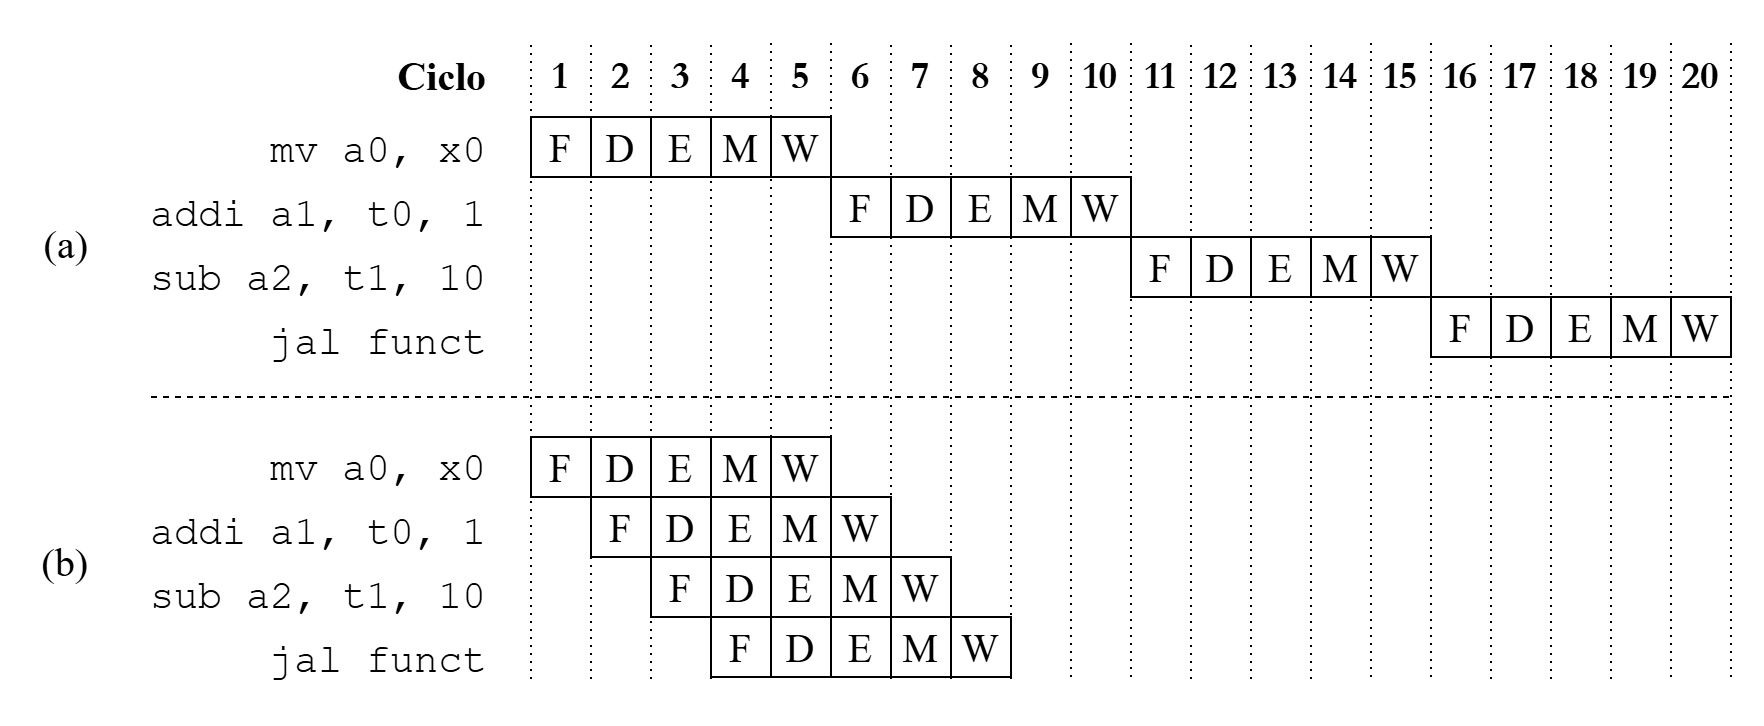
\includegraphics[width=1\linewidth]{res/img/diagramas/cap05singleVSpipelined/singleVSpipelined.png}
  \caption{Ejecución de un programa en un computador con diseño monociclo (a) y segmentado (b)}
\end{figure}

Esta técnica conlleva una mayor complejidad arquitectónica y el surgimiento de una serie de riesgos o \textit{hazards} generados bien por las dependencias de datos entre las instrucciones de un programa (ver Figura 5.2), o bien por la ejecución de instrucciones de control que pueden o no alterar el flujo de ejecución de este (ver Figura 5.3). En función de las decisiones de diseño que se tomen para abordar la problemática que representan estos fenómenos, su aparición desembocará la introducción de detenciones (\textit{stalls}) en el flujo de ejecución, o la necesidad de incluir en el diseño mecanismos adicionales como el \textit{forwarding}, consistente en el conexionado de determinadas señales de datos o de control hacia etapas anteriores en el pipeline.

\vspace{0.2cm}

\begin{figure}[ht]
\centering

\setlength{\fboxsep}{10pt}
\setlength{\fboxrule}{1pt}

\fbox{%
\begin{minipage}{0.95\textwidth}
\centering

\begin{minipage}{0.22\textwidth}
\centering
\texttt{add \textcolor{purple}{x1}, x2, x3}\\
\texttt{sub x4, \textcolor{purple}{x1}, x5}\\
(a)
\end{minipage}
\hfill
\begin{minipage}{0.22\textwidth}
\centering
\texttt{add \textcolor{purple}{x1}, x2, x3}\\
\texttt{add \textcolor{purple}{x1}, x4, x5}\\
(b)
\end{minipage}
\hfill
\begin{minipage}{0.22\textwidth}
\centering
\texttt{add x4, \textcolor{purple}{x1}, x2}\\
\texttt{add \textcolor{purple}{x1}, x3, x5}\\
(c)
\end{minipage}

\end{minipage}%
}

\caption{Ejemplos de riesgos de datos. 
(a) Dependencia RAW: la instrucción \texttt{sub} deberá esperar a la escritura de resultados por parte del \texttt{add} en \textcolor{purple}{x1} para elaborar un resultado coherente.
(b)(c) Dependencias WAW y WAR respectivamente: ambas instrucciones pueden operar con el registro \textcolor{purple}{x1} sin que ello suponga una pérdida de coherencia en los datos.}
\label{fig:dependencias_riscv}

\end{figure}

\vspace{+0.5cm}
\begin{figure}[h]
  \centering
  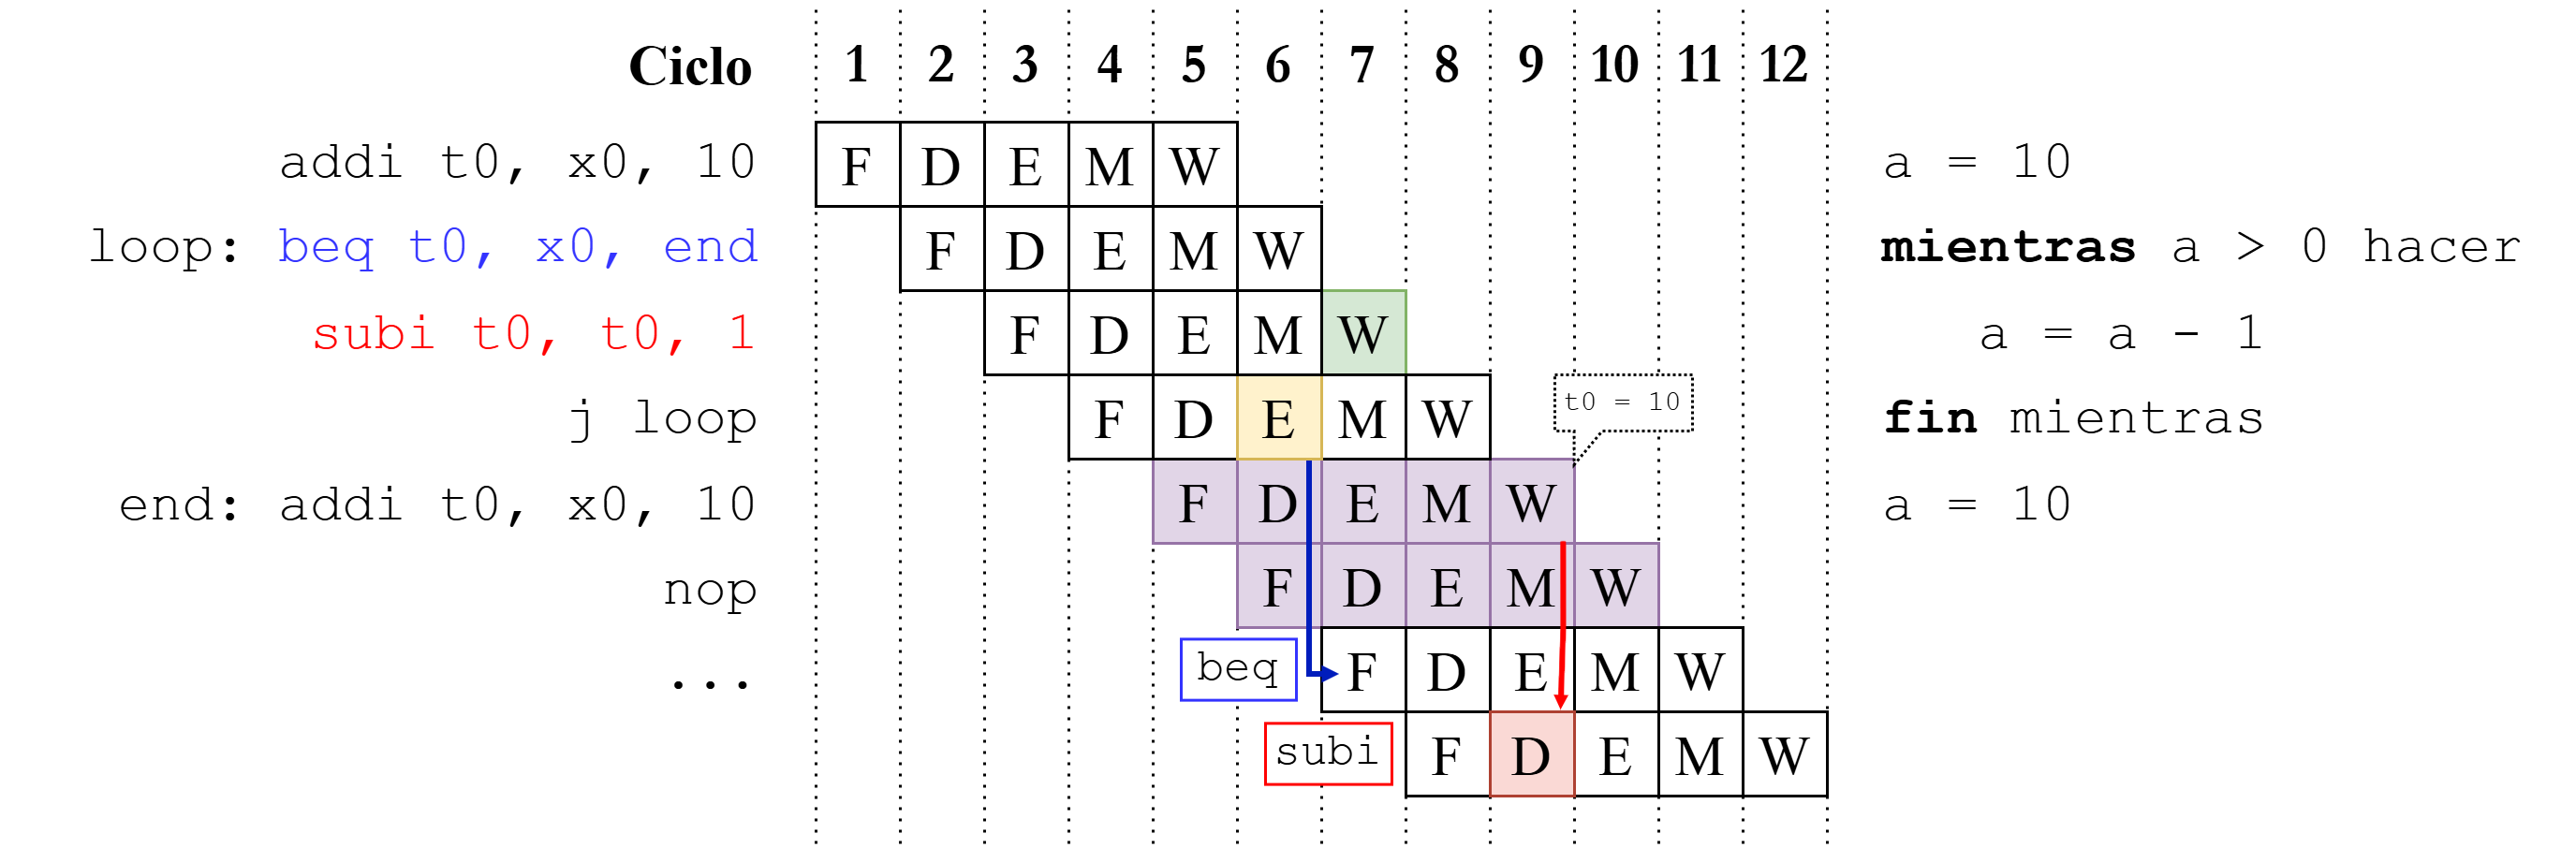
\includegraphics[width=\linewidth]{res/img/diagramas/cap05riesgoControl/cap05riesgoControl.png}
  \vspace{+0.05cm}
  \caption{Representación del flujo de ejecución de un programa sobre una arquitectura segmentada sin mecanismos para resolver riesgos de control. Nótese que el resultado de la instrucción de resta (\texttt{subi}) se escribe (writeback señalado en color verde) en el banco de registros ántes incluso de evaluar la condición en la instrucción de salto, dejando el valor del registro \texttt{t0} en un estado inconsistente. Además, dado que el destino del salto de la instrucción \texttt{jal} no se calculará hasta su ejecución, habrá dos ciclos en los que se introducirán las dos instrucciones inmediatamente posteriores (señaladas en color morado), una de las cuales reinicia el valor de la variable \texttt{a} haciendo que el bucle no tenga final. El resultado de la instrucción \texttt{subi} en la primera iteración se sobreescribe con el del segundo \texttt{addi}.}
\end{figure}

No obstante, y a pesar de estas limitaciones, la segmentación de instrucciones permite obtener un speedup teórico igual al número de etapas en que se haya decidido segmentar la arquitectura, teniendo siempre en cuenta que aspectos como la presencia y resolución de los riesgos mencionados, la latencia en los accesos a memoria o el tiempo desigual entre los caminos críticos de las diferentes etapas, impedirán alcanzar ese rendimiento máximo ideal.



%%%%%%%%%%%%%%%%%%%%%%%%%%%%%%% Primera aproximación %%%%%%%%%%%%%%%%%%%%%%%%%%%%%%%%
\section{Primera aproximación}

% TODO: Ya veré en qué punto del capítulo meto lo de las decisiones de diseño relativas 
% a la integración de los registros de etapa...
En un primer momento se optó por aplicar un enfoque incremental en lo que respecta a la inserción de los registros de etapa. No obstante, este enfoque se aplicó tan solo en la integración del primer registro de etapa para separar la fase de \textit{fetch} del resto del pipeline. Esto fue así puesto que, de haber seguido integrando registros de etapa uno a uno, verificando el funcionamiento del núcleo con dos, tres y cuatro registros, el proceso de desarrollo se hubiera dilatado en el tiempo más allá de lo deseado inicalmente. Esto hubiera sido así puesto que, para cada una de las integraciones de un registro de segmentación a partir de aquel que separa las fases de \textit{fetch} y decodificación, hubiera sido preciso diseñar una solución distinta al problema que generan las dependencias de datos y de control entre las instrucciones que atraviesan el pipeline.

Es por ello por lo que se consideró que resultaría más eficiente integrar los registros de segmentación siguientes al de \textit{fetch}-decodificación a la vez, desarrollando una única solución al problema generado por las dependencias de datos y de control.



%%%%%%%%%%%%%%%%%%%%%%%%%% Segmentando el resto del pipeline %%%%%%%%%%%%%%%%%%%%%%%%%%%
\section{Segmentando el resto del pipeline}

